\documentclass[manuscript, nonacm]{acmart} 
\title{Real World Geometry} 
\subtitle{Supplimental Geometry Instruction via an Augmented Reality Application} 
\author{Tong Chu}
\author{Connor Onweller}
\author{Jie Ren}
\usepackage{natbib}
\usepackage{graphicx}
\usepackage[toc,page]{appendix}

\makeatletter
\let\@authorsaddresses\@empty
\makeatother


\begin{document}

\maketitle

\section{Introduction}
\label{sec:introduction}

Geometry is an essential area of mathematics but considered difficult by kids
when they first access it in school.  By learning geometry, students may be able
to identify shapes and space around them.  However, kids know 3D shapes even
before going to school.  They intuitively investigate and interact with 3D
shapes/objects by exploring it, since everything around us is three-dimensional.
Then they go to school and learn to write and draw in two dimension
\cite{AR-3D-geometry}.  It is getting more challenging that after kids already
know that everything at school is 2D, they need to learn 3D geometry.
Unfortunately, traditional teaching methods failed to assist kids to smoothly
transition from 3D to 2D and go back to 3D.  In addition, due to kids’ own
cognitive gap between 2D and 3D shapes, it is hard for them to get knowledge of
geometry.  Therefore, it is the time for teachers/parents seeking a new
perspective to help kids with geometry learning.

In recent years, digital technology is employed in education since technology
tools are very interesting and engaging for kids \cite{game-based,
using-games-learning, game-based-learning, adaptive}. Augmented Reality (AR) is
one of the most explored and successfully used technologies.  According to
Piaget’s Constructivism theor \cite{psych-child}.  kids easily acquire new
knowledge if learning occurs in a specific context and is embedded in a physical
environment.  Thanks to AR, it allows users to be completely immersed inside a
synthetic environment, which makes learning more effectiv
\cite{situated-learning}.  Since AR permits to create interaction experiences
that are enhanced by the overlapping of information between virtual and real
objects, it improves the involvement of kids during their learning proces
\cite{AR-support-geometry}.

In 1999, van Hiele proposed a theory named “Levels of Geometric Thinking”, which
claimed that the geometric thinking could be divided into four levels, from
“lowest” to “highest” were: visual level (figures were judged by their
appearance), the descriptive level (figures were the bearers of their
properties), the informal deduction level (the properties of figures were
logically ordered) and the deduction level (used axioms, definitions, theorems
to identify figures \cite{developing-geometric-thinking}.  The best way to help
kids develop geometric thinking was to follow the sequence from lowest level to
the highest, i.e. developing thinking from the visual level and gradually
transition to the descriptive level, at the end reaching to the final deduction
level.

\section{Problem Statement and Related Work}

\subsection{Probelm Statement}

Due to the reason that geometry plays an essential role in math but is too
abstract for kids to learn, a new method which helps kids to build a connection
between 2D and 3D geometry, develop spatial imagination and the capacity of
abstraction geometry is urgent. Augmented Reality (AR), as a promising
technology, allows kids to be completely engaged in the environment. Moreover,
some AR-based multimedia is able to display both 2D and 3D objects by showing
every part of the objects in detail \cite{use-of-geometry-media}.  Based on the
above reasons, our goal for the project is to develop an AR app that makes
tangible the geometric properties they learn about. Each level of the app will
include three steps (based on van Hiele’s “Levels of Geometric Thinking”): (1)
visual identification (2) kids interact with their environment in AR to discover
geometric ideas (3) combines conceptual content (definitions and
characteristics) with procedural content (applying formulae and calculus). Our
app will provide a new perspective for kids to better understand geometry, and
increase geometry motivation and mathematics with AR.

\subsection{Related Work}

There are some AR based geometry learning applications. For example, Arloon
Geometry is an application designed for middle school students (> 11 years old)
to improve their 3D thinking skills. This application features 3D models with AR
for most geometric shapes, such as pyramids, prisms etc., and the pupil
interacts with the game by viewing geometric shapes from all angles and listing
their properties and the formulae that define their area and volume. However,
this application requires an Android system and is not suitable for younger
kids. Shapes 3D is another AR based application which allows students to
interact with real 3D shapes by placing solids everywhere and even rotate a 3D
shape to better understand the geometric shapes. However, due to the complexity
of this application, it does not implement AR technology with detecting
objects. Kyle Wang and Ray Patt’s last year’s project, Real-World Geometry,
includes three steps: kids identify shapes through visual identification, using
AR interact 3D geometric shapes to identify them, and the highest level is
interacting with the surrounding environment to better understand geometric
concepts. This application is very promising, but due to time limitations, they
only applied to three simple shapes, and did not reach to the highest level,
deductive thinking level.

\section{Need Finding}

We plan to perform need finding using interviews with domain experts.  Here we
define domain experts as teachers that have experience working with K-5 children
and that have experience teaching basic geometry. We will send out an email to
education majors at the University of Delaware. Our goal is to get an sufficient
understanding of what material students struggle with the most and therefore get
an understanding of what topics our app should address. We also want to get
guidance for how to best communicate instructions to these students and what
techniques tend to keep them engaged. A sample interview protocol is included in
appendix \ref{appendix:interview}.

\section{Prototyping}

We first used wireframe prototype via Miro. Describe the process via which users
will interact with our application.  In doing so we focus more on breadth of the
features we covered rather than depth; we aim to show the majority of the
features involved in our applicaiton, but our prototype will not impliment any
real functionality. Our initial prototype can be found in appendix \ref{appendix:prototype}.

\section{Implimentation}

We consider the spatial relationship between items on the page and structure the
page according to importance. We carefully place the items which helps kides
draw attention to the most important information,(the geometry shapes and
equations) and aids in scanning and readability.

To improve the prior work and design, we plan to use color and texture
strategically. We use color, light, contrast, and texture to focus or shift
users attention to the project. The different sizes, fonts, and arrangement of
text help improve scannability, legibility, and readability to ensure that the
system communicates and always notify users of location, operation, status
changes or errors when they pass along the tasks.

In conclusion, we use various UI elements to communicate status and subsequent
steps when necessary can reduce user frustration.

We are going to use matlab to refine the coding that prior team have done, and
also we will develop the application to improve user experience in terms of
accessibility, readability, entertainment value.

One challenge we may face is the need to balance our goal of adding new and
interesting features to the existed application with our desire to maintain a
simple simple and easy to interface for our users.

We are building a mobile app, and are currently targeting only
iPhones. Hopefully will eventually be able to expand to android phones as
well. We view a mobile app as the best medium for this project, as children will
likely be familiar with mobile apps, and mobile app will allow us to easily
access a camera which will be necessary for the AR functionality that the app
will utilize.

\section{User Study / Evaluation}

The goal of our user study will be to assess the effectiveness of our project
and motivate future changes that could be made to the app. Will perform this in
one human subjects study where we will collect quantitative and qualitative
information about the users' experiences using our application.

We will evaluate the following hypothesis question: Does usage of our
application improve student performance on geometry assessments when compared to
traditional teaching methods?

We will recruit elementary school students to participate in our study (likely
through family/friends for convenience). The students will be asked to take a
short geometry pre-assessment. We will conduct a between subjects experiment
where students are exposed to one of two conditions: (1) a traditional teaching
method simulated through a short video that explains geometric concepts (this is
our baseline condition) (2) our Real World Geometry application. After this we
will assess students from both groups on the same geometry assessment. We will
then compare score improvements for each group, look to see if there is a
significant difference between them. We will ask the students assigned to
condition 2 to take a brief survey, to get a better understanding of their
experience using our application.

\section{Alterative Approaches}

We planned to use ARKit 2 and paired it with Unity, however, it also has
downsides, e.g. only supporting macOS and iOS systems. We prepared some backup
plans: first, we can build AR with Vuforia with Unity or ARCore with Unity,
because we can run it on Android system; second, we can also try ARToolKit5,
since it is fast, intuitive and cross-platform, and can be run on macOS, iOS,
Linux, Android or Windows.

\section{Timeline and Deliverables}

\begin{enumerate}
    \item We finished our storyboard during the week of October 25, 2021. (All the
    member)
    \item We discussed and finished our first draft proposal (also presented in
    class) during the week of November 1st, 2021. (All the members)
    \item We plan to write our second draft proposal (through word) during the week
    of November 15, 2021. (All the members involved discussion, each member was
    responsible for at least two parts and at the end modified and finished
    together)
    \item We plan to write and run the code during Thanksgiving week (November 22,
    2021) (Jie and Connor) and also design and work on our survey, observations
    part. (All the members)
    \item We plan to finish the detailed user study/evaluation part during the week
    of November 29, 2021. (All the members)
    \item This project is expected to be completed by December 17, 2021. (All the
    members)
\end{enumerate}

\section{Biographies}


\begin{description}
\item[Jie Ren] \hfill
  \begin{description}
    \item[Field of Study] Computer Science
    \item[Role] Developer, Coding, Project Manager
  \end{description}
\item[Connor Onweller] \hfill
  \begin{description}
    \item[Field of Study] Computer Science
    \item[Role] Developer, Research Informant
    \item[Interests] Computer Accessibility, Computer Vision, Software Engineering
  \end{description}
\item[Tong Chu] \hfill
  \begin{description}
    \item[Field of Study] Biomedical Engineering
    \item[Role] Developer, product designer, information search assistant 
    \item[Interests] Medical Design experience (Patent Pending)
  \end{description}
\end{description}


\bibliographystyle{ACM-Reference-Format}
\bibliography{references}

\begin{appendices}

  \section{Interview Protocol}
  \label{appendix:interview}
  \begin{enumerate}
  \item \textbf{Introduction}

    Hello, my name is \rule{1cm}{0.15mm}.  I am a student at the University of
    Delaware studying the role that augmented reality software can play in
    geometry education.  I am looking to gain some insight on your experience
    teaching students geometry.

  \item \textbf{Questions}

    \begin{itemize}
      \item What grade do you teach?
      \item How many classes do you typically spend covering geometry per year?
      \item Do you enjoy teaching geometry?
      \item Is teaching geometry ever difficult? If so, what kind of things make
        it difficult?
      \item Do you ever use resources like videos, websites, or games to help
        teach? If so, do you ever use any of these to help teach geometry?
      \item Could you see a geometry phone game as something that could be a
        helpful supplimentary tool for teaching?
      \item What topics would you think such a game should cover?
      \item How do you best communicate instructions for students to complete
        activities, assignments, and games? What types of considerations should
        be made when doing so
    \end{itemize}

  \item \textbf{Conclusion}

    Thank you for participating in this study. We will send you an update when we
    complete our paper.
  \end{enumerate}

  
  \section{Prototype}
  \label{appendix:prototype}
  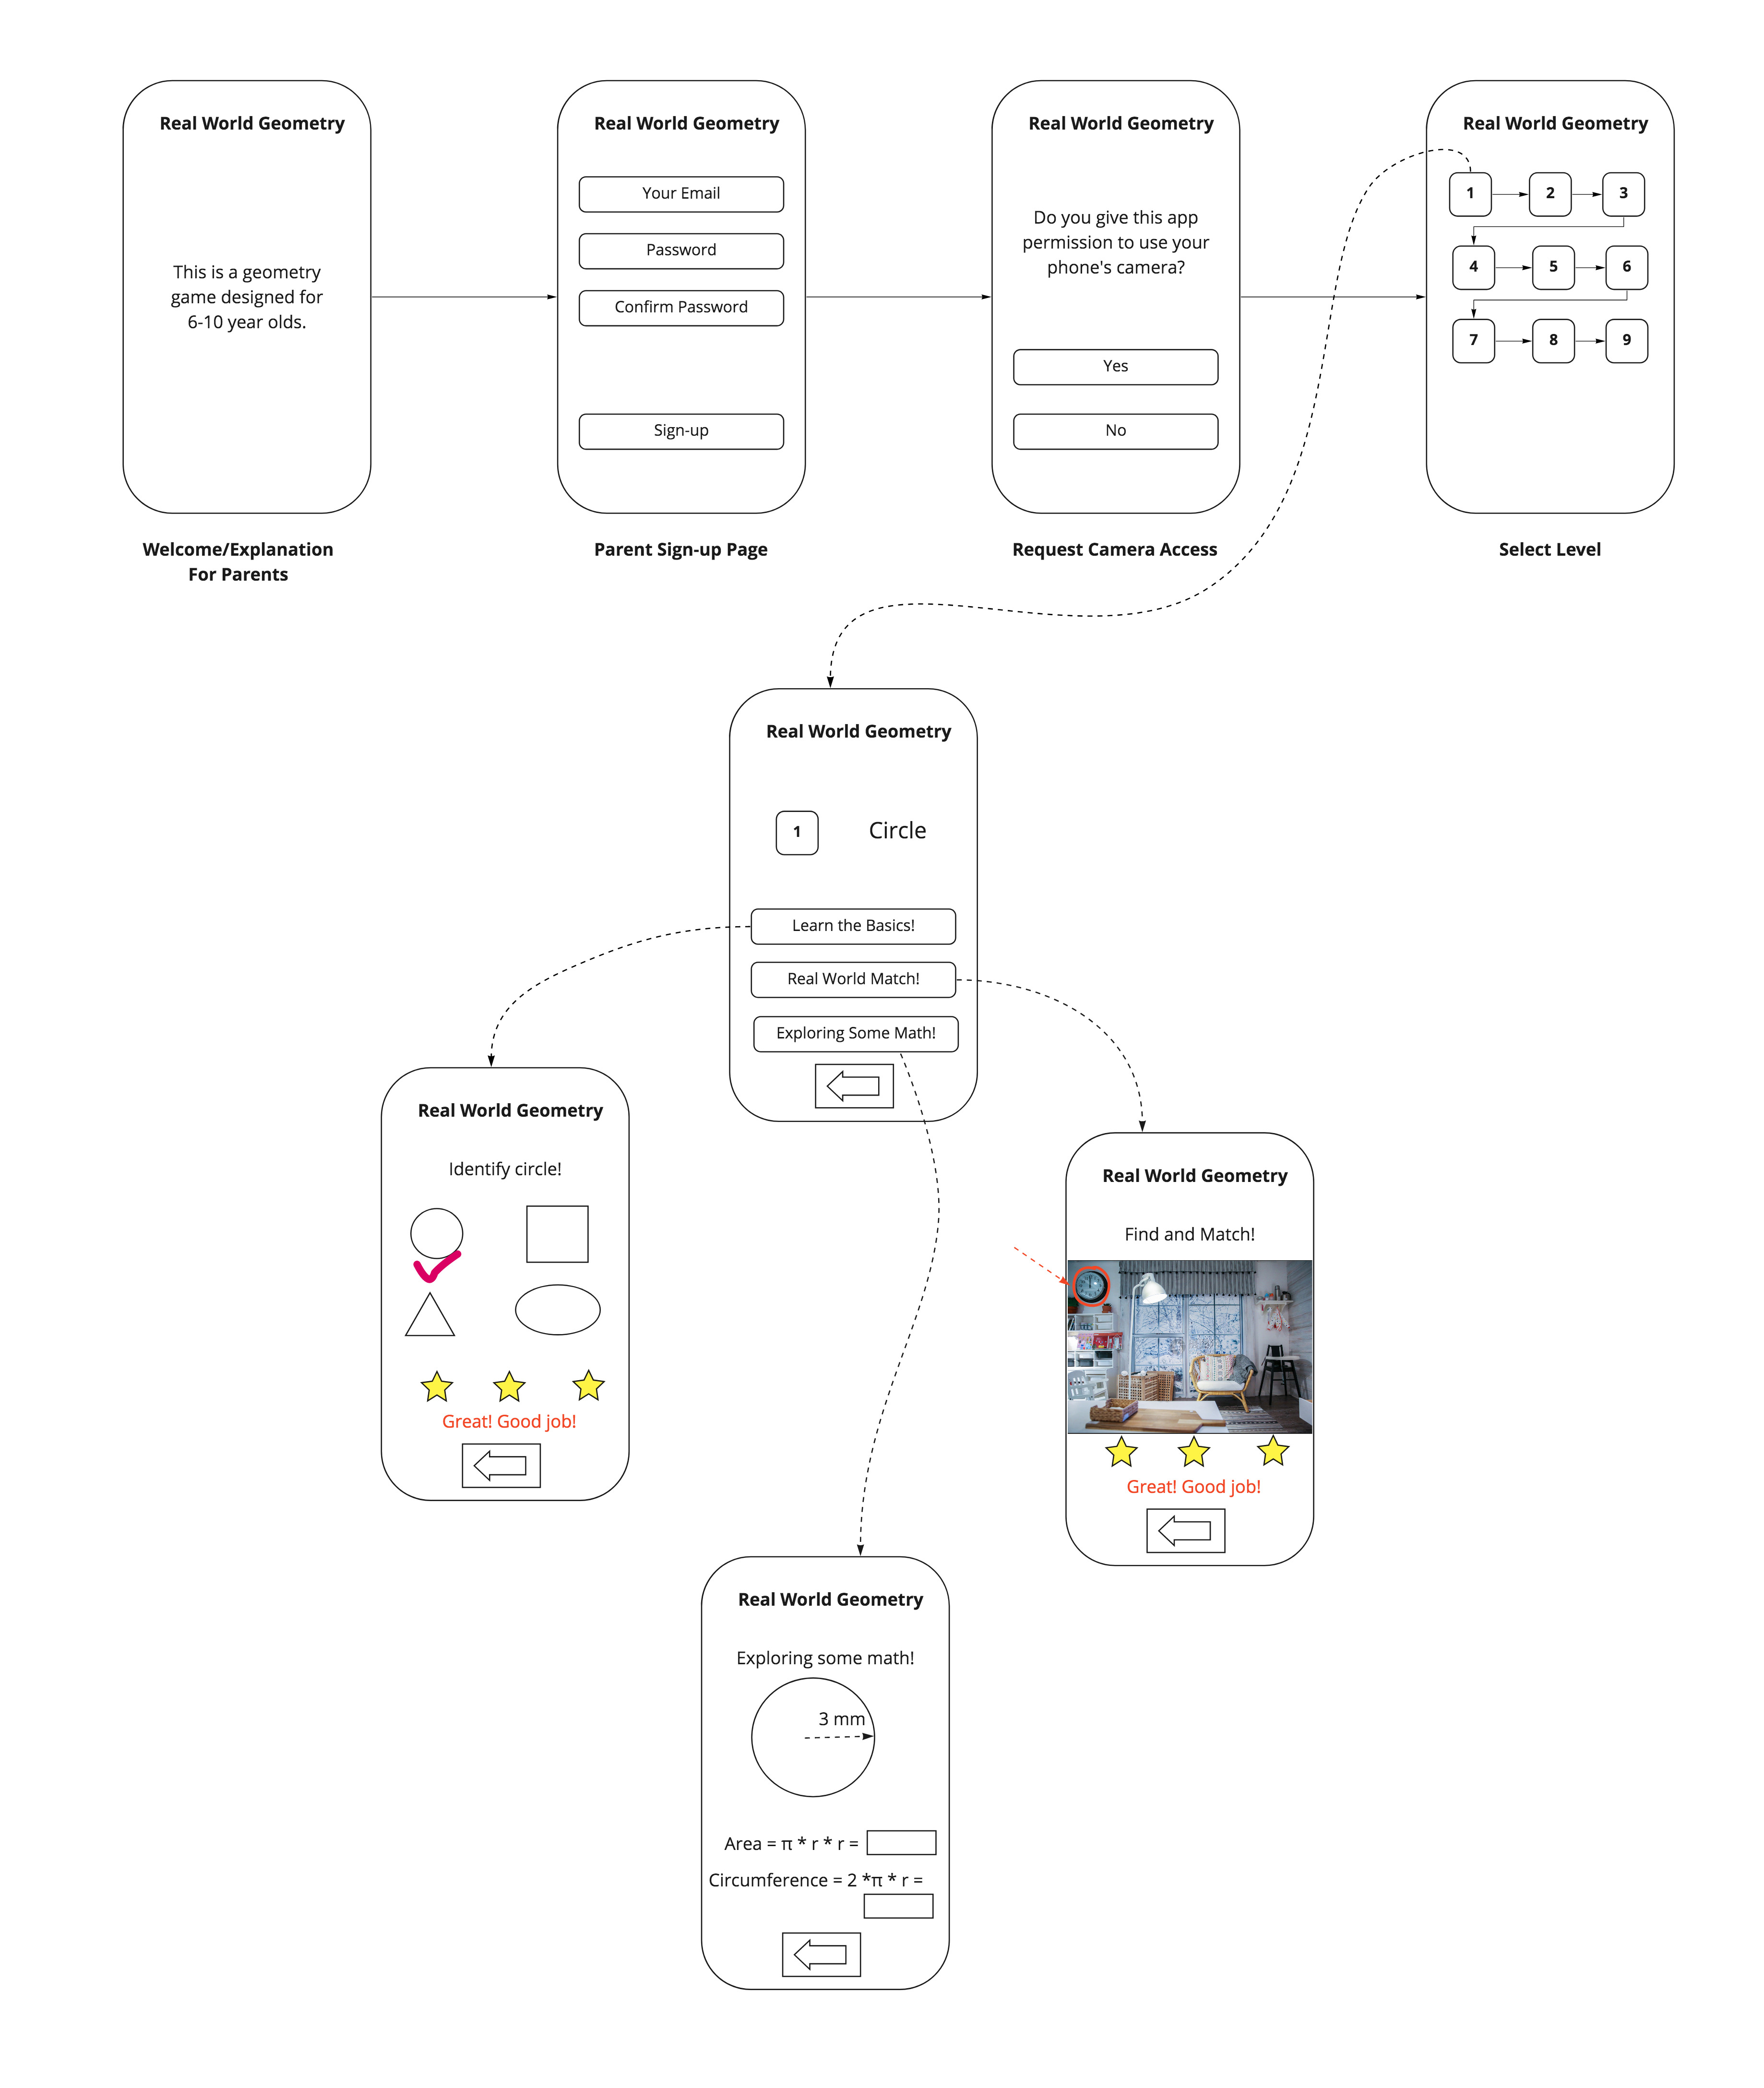
\includegraphics[width=\textwidth]{prototype.jpg}

\end{appendices}

\end{document}
